The system consists of a thrust vectoring rocket with an Inertial measurement Unit (IMU) GY-87.
Multiple physical and software constraints have to be taken into account when implementing the designed controller. For the software part, the controller is implemented in same manor as the inverted pendulum, with the variables values changed to fit the rocket controller.  

\section{Implementing Sensors and Servomotors}
The response time of the sensors are an important feature when ensuring the stability of the rocket. It can not be too slow, otherwise the system will react to late to angle variation. The servomotors system dynamics are described in \autoref{ssc:Servomotors}. The implementation was done by implementing the Servo library in Arduino, and the position is set by a writing a position between -180 and 180 degrees trough the Servo.Write(); function. 

 I$^2$C or Inter-Integrated Circuit, which is the protocol used to link the Arduino and the IMU. The I$^2$C as working on the hardware wires for operation.
\begin{itemize}
	\item SDA (Serial Data Line): Bidirectional data line
	\item SCL (Serial Clock Line): Bidirectional clock synchronization line
\end{itemize}
They are connected to the dedicated I$^2$C pins on the Arduino.
The gyroscope/angle sensor needs to write 14 bytes into the Arduino register. The code to use the MPU 6050 was done by Brainergizer \cite{web:gyro_angle}. Since the gyroscope has an internal clock of 1MHz \cite{datasheet:MPU-6050}, the sampling time for the angle sensor is $\frac{14 \cdot 8}{1 \cdot 10^{6}} = 1,12 \cdot 10^{-4}$ seconds giving a sampling rate of approximatively 8,9 KHz. The processing time of the 16 MHz micro-controller is considered insignificant, since there is no time-intensive sensor processing tasks in the code. 

The Arduino produces a PWM signal to control the servo angle. The servomotor standard integrated controller interprets the angle command based on the duty cycle. 0\% is - 180$^{\circ}$ and 100\% is + 180$^{\circ}$. These PWM signals needs to be passed to the PSU board where the servo connector are seen cf. section \ref{sec:PowerToThePeople}.

To control the rocket and to fire it safely, 3 different PCB (Printed Circuit Boards) were designed. A logic board, a Power Supply Unit (PSU) and an electric igniter. The logic board and the PSU are stacked on top of each other and the battery is inserted between the two cards to optimize space. All cards schematics are available in the included  in folder "/Attachment/Implementation/Rocket/Rocket PCB schematics".

\subsection{Logic Board}
The logic board hosts the Arduino Nano micro-controller, the battery connector, the servo output, the IMU and four indicator LEDs.

\begin{figure} [h]
	\centering
	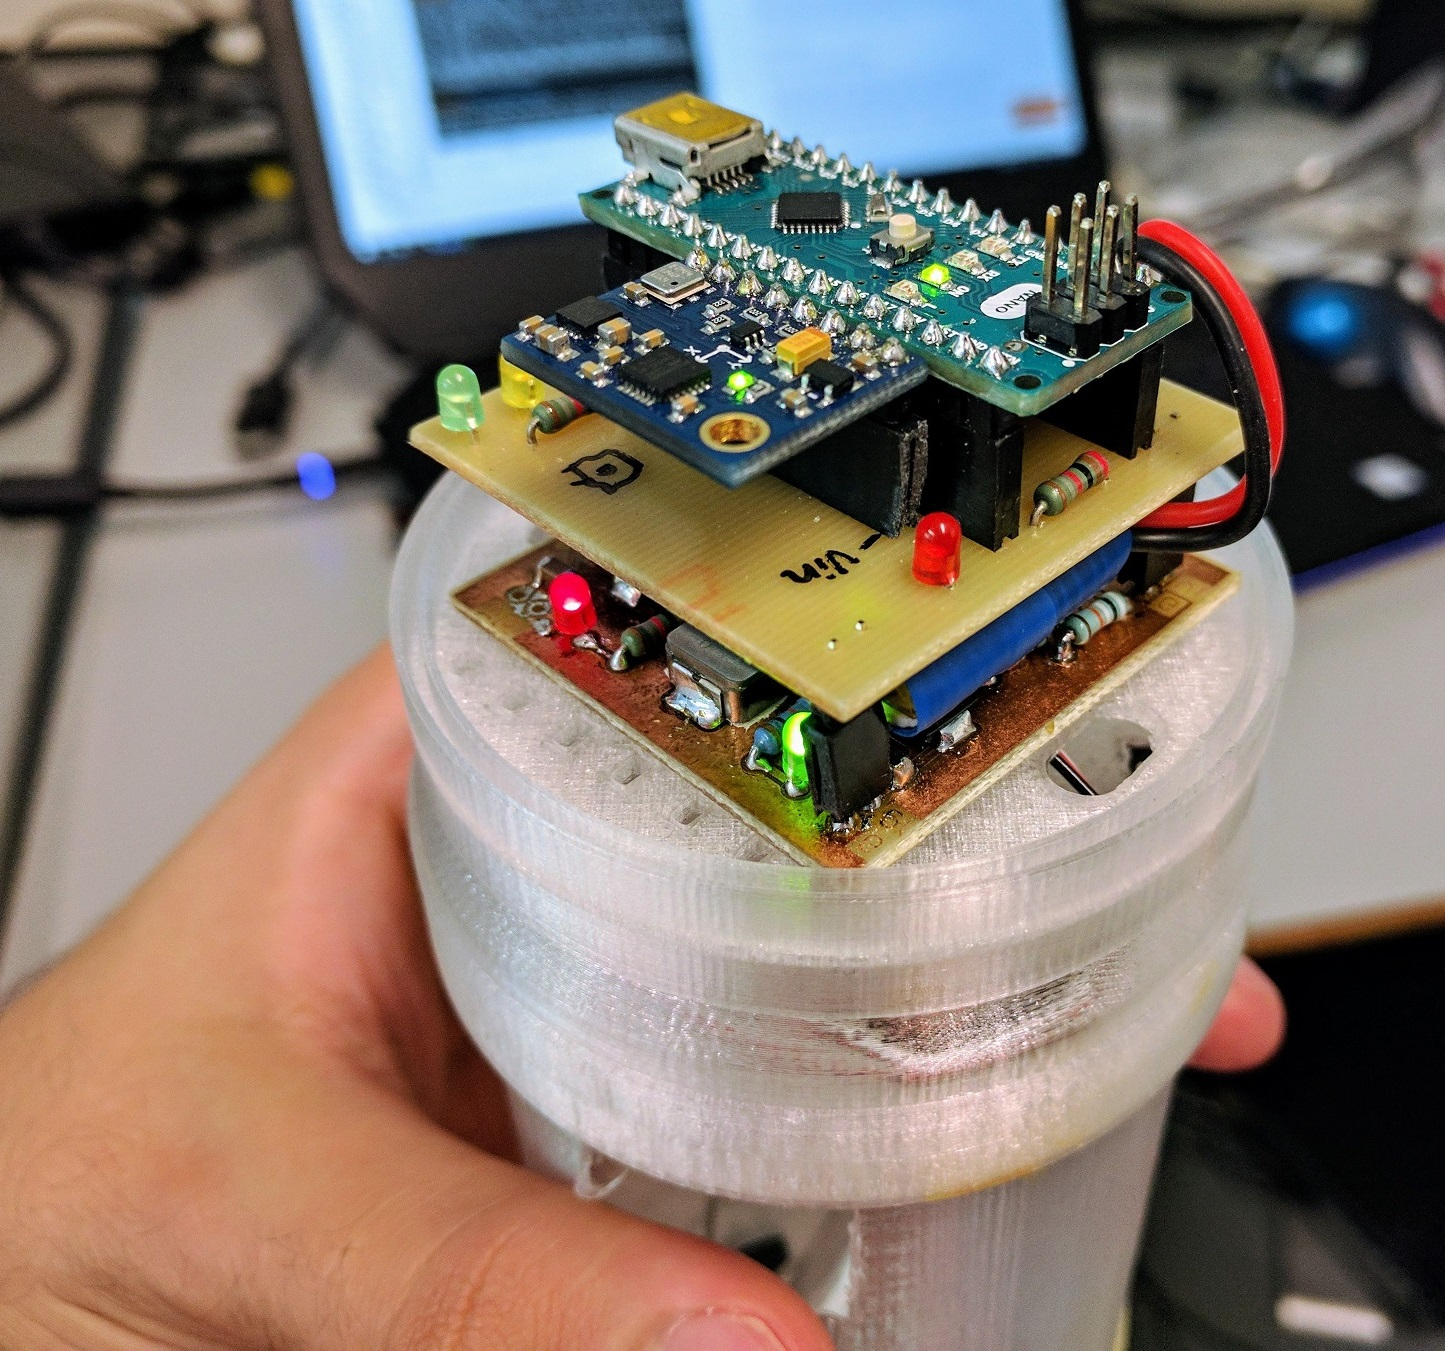
\includegraphics[width=0.7\linewidth]{figures/Rocket/implementation/assembled_PCBs.jpg}
	\caption{PCB stack assembled with the logic board on the top.}
	\label{fig:PCB_stack}
\end{figure}

The battery voltage is directed towards an analogue input on the Arduino. This is to enable a batteri check for seeing the charge state, and light a LED when the battery is below a threshold voltage. \\
The 3 other remaining LED indicators are provided for debugging purposes only.
The battery input is then passed by a connector to the PSU below, that provides the 5 V rail to power the Arduino and the IMU.

\subsection{Power supply}\label{sec:PowerToThePeople}
The rocket is electrically powered by a single cell 3,7 V, 680 mAh LiPo battery. These batteries are lightweight, rechargeable and available in small form factors that fitted perfectly the rocket's size. \\

\begin{figure} [h]
	\centering
	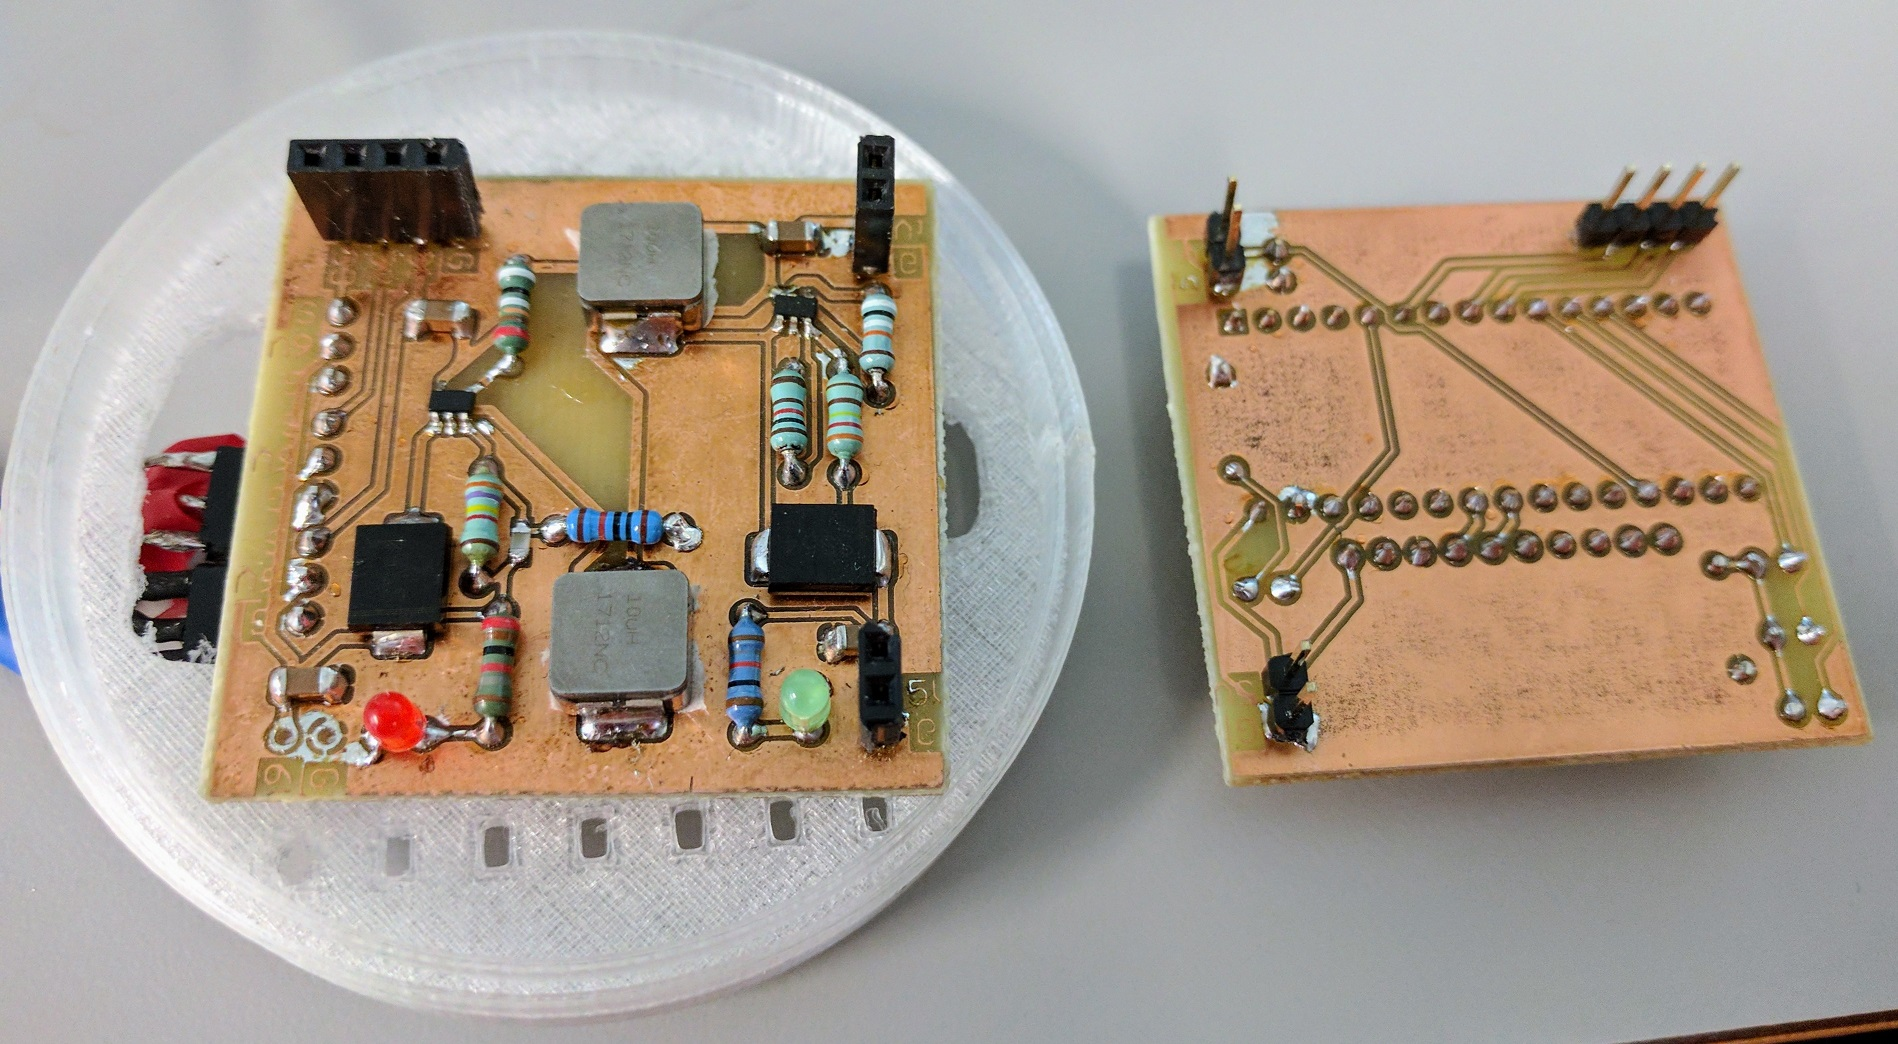
\includegraphics[width=0.7\linewidth]{figures/Rocket/implementation/psu_board.jpg}
	\caption{PCB stack disassembled, with PSU on the left.}
	\label{fig:PSU_board}
\end{figure}

The logic components and the actuators must be very well separated since if they are not, a current draw spike on the actuator side could take all available power and shut down the logic components for a brief amount of time. This would cause them to reset, and the rocket to go out of control. \\
Since the logic and actuator parts of the power supply needs to be separated, two different power supplies were created on the same board (with common ground). \\
The logic side needs a 5 V rail to function. The components are all powered by their Vin pin, which mean that they had a voltage stabilizer included. The 5 V output was set to 5,2 V to compensate for the losses in the stabilizing circuit. \\
The actuators, namely the pitch and roll servos is nano servos, which implies a small size and light weight. As most standard servo can operate from 4.8V to 6V, they will be faster and have more torque at higher voltage. The second power supply output was set to 6V to give the maximum torque. The servo test in \autoref{ssc:Servomotors} determined these supply conditions, based on testing the speed at different voltages. The servo connectors have 3 pins, a PWM input was connected to the PWM output from the arduino, Vin was the 6V from the PSU, and the last pin is ground. \\
The PSU 5 V rail was found to work at an input voltage as low as 3,6 V. The LED low battery indicator threshold was set to 3,65 V.

\subsection{Igniter}
The igniter plugs that were implemented needed a 6V to 9V supply to ignite. 3-cell LiPo batteries are very common in the university, so the power was taken from a LiPo balancing plug, thus only using 2 cells to get 7,4 V nominal voltage. The board is a switch mechanism, the ignition needs to be armed first by flipping a switch before pushing the "fire" button. The PCB also features a protection capacitor, a buzzer and LEDs for user feedback.

\begin{figure} [h]
	\centering
	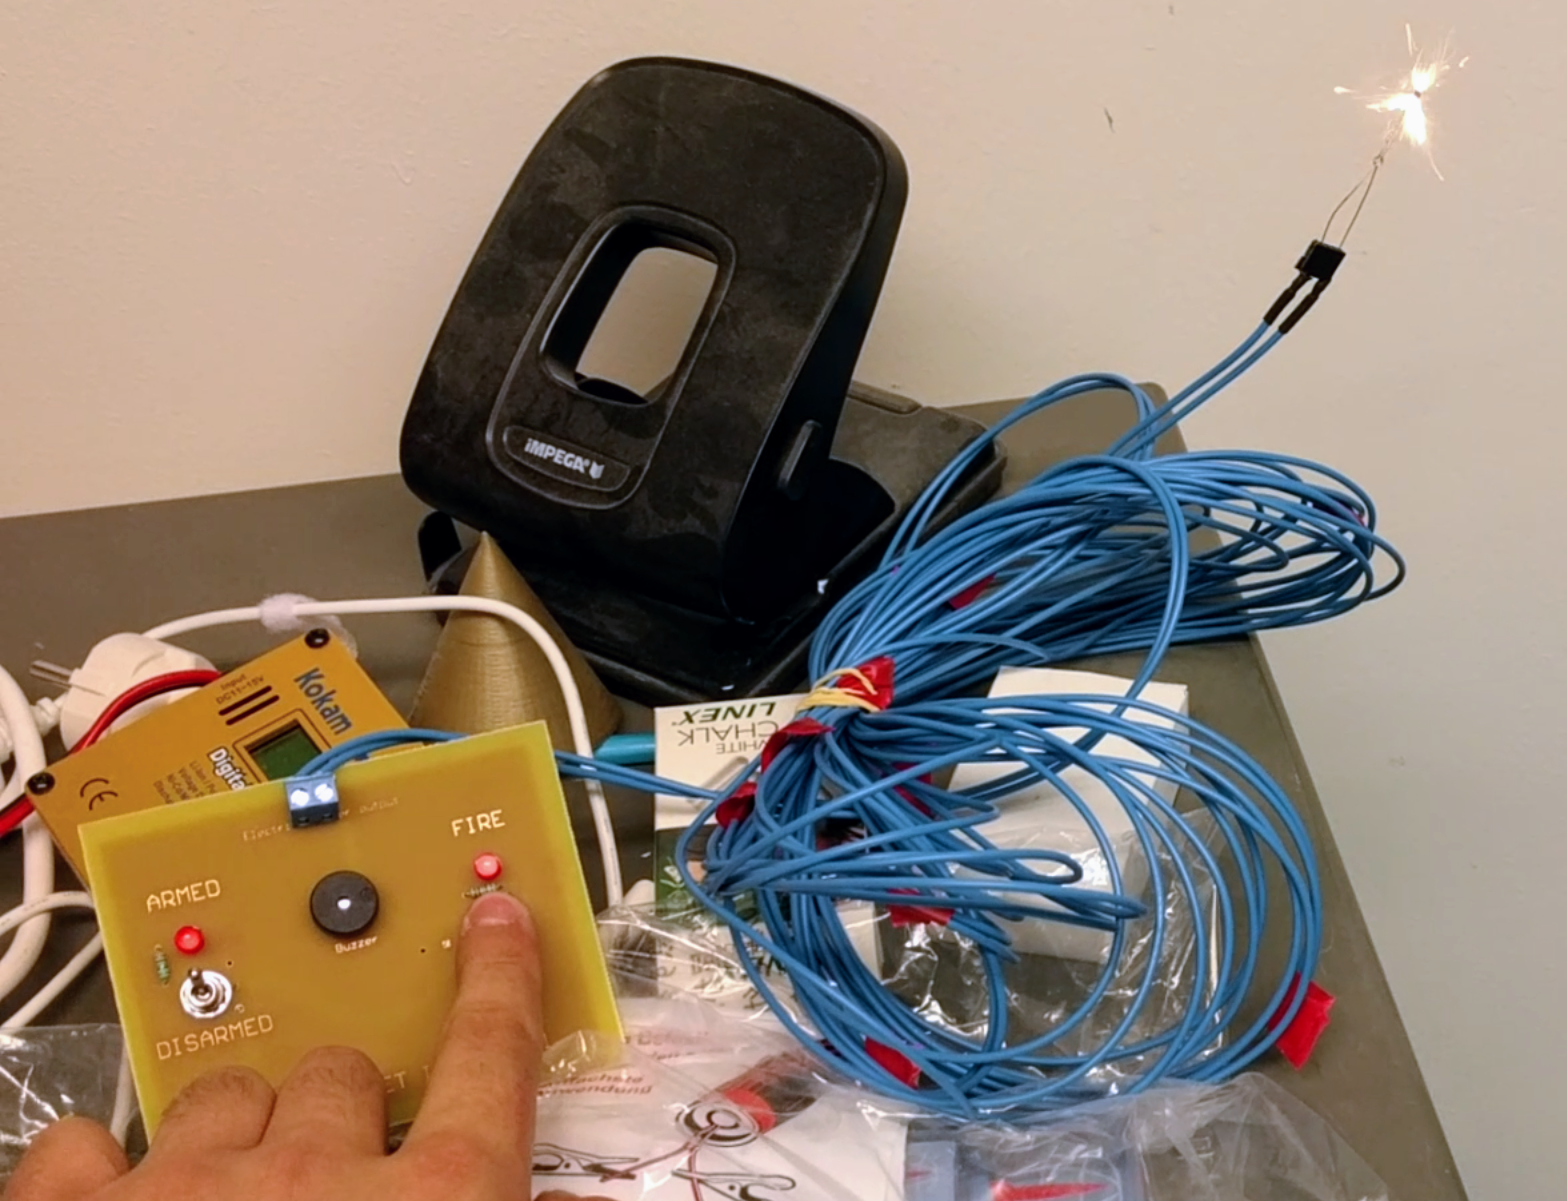
\includegraphics[width=0.9\linewidth]{figures/Rocket/implementation/igniter_PCB.png}
	\caption{Lighting an igniter with the PCB.}
	\label{fig:igniter_board}
\end{figure}

The hardware implementation was completed and gave the possibility to implemented the controller trough Arduino software.
\newpage
\section{Rocket Software}
The software implemented can be seen in the Arduino Software attachment folder "/Attachment/Implementation/Rocket/Controller_code_rocket/Controller_Rocket.ino". A software flowchart is obtained to give a structural overview, which can be seen on figure. The principle is to determine the pitch and roll trough the IMU and then control the servo motor to a opposite angular reaction to stabilize the rocket.  

\begin{figure}[htbp]
	\centering
	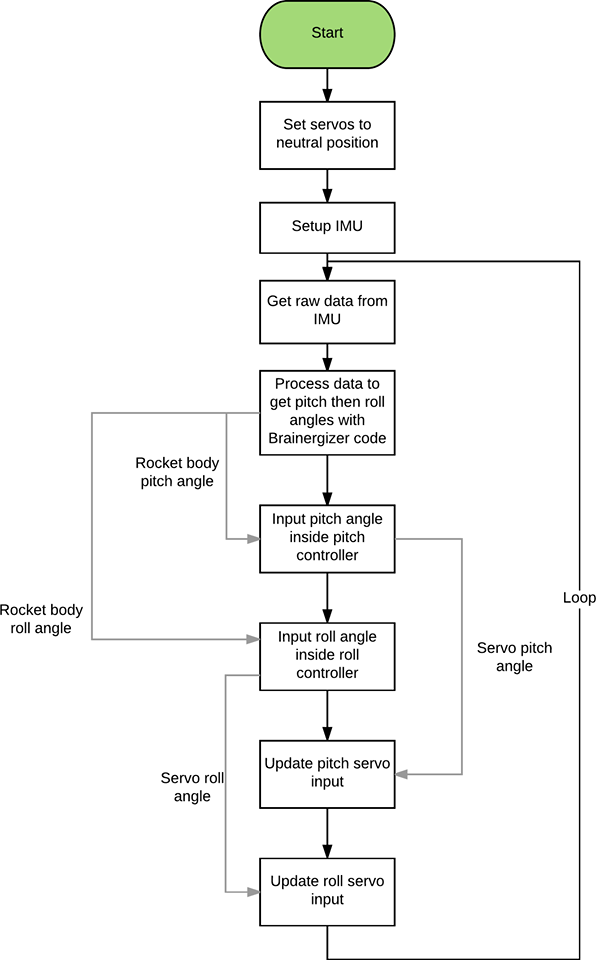
\includegraphics[width=0.6\linewidth]{figures/Rocket/implementation/FlowRocket}
	\caption{Flowchart of rocket software.}
	\label{fig:igniter_board}
\end{figure}

\newpage
\section{Flight test}
The rocket was tested without the thruster to visually confirm if the system was behaving correctly. A video of this test is included in attachment folder "/Attachment/Implementation/Rocket/rocket_controller_check". The controller inclined the thruster in the correct direction according to the rocket's tilt. A flight test was planned but delays in the rocket's construction did not allow to make the test safely.
Strings would have been attached radially to the center of gravity of the rocket, and wrapped around two sticks three meters apart. The wires would have been made long enough so the rocket would have been hovering slightly over the ground and then the truster would be fired. Filming the flight and logging the angle data on the Arduinos memory could have shown the angle of  the rocket during flight.